\subsection{Theorems}

\begin{frame}{Theorems}

    \begin{center}
        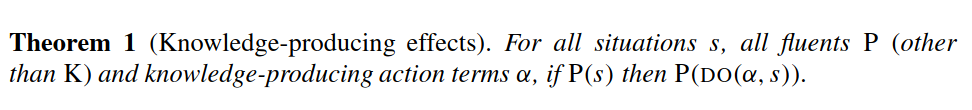
\includegraphics[width=0.7\textwidth]{assets/theorem1.png}
        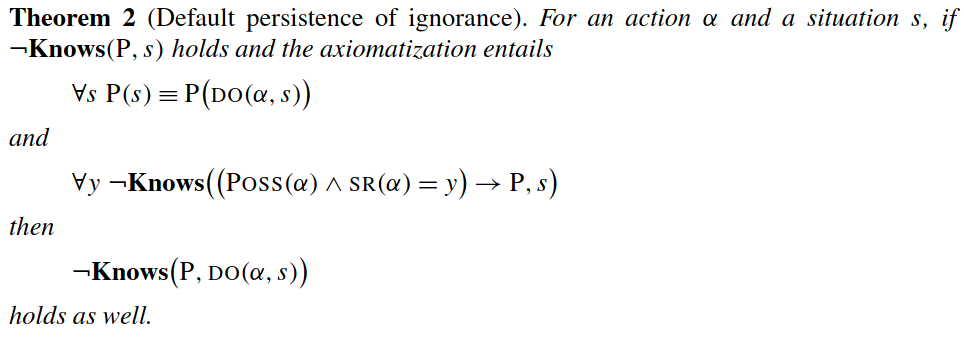
\includegraphics[width=0.7\textwidth]{assets/theorem2.png}
    \end{center}

\end{frame}    

\begin{frame}{Theorems}
    \begin{center}
        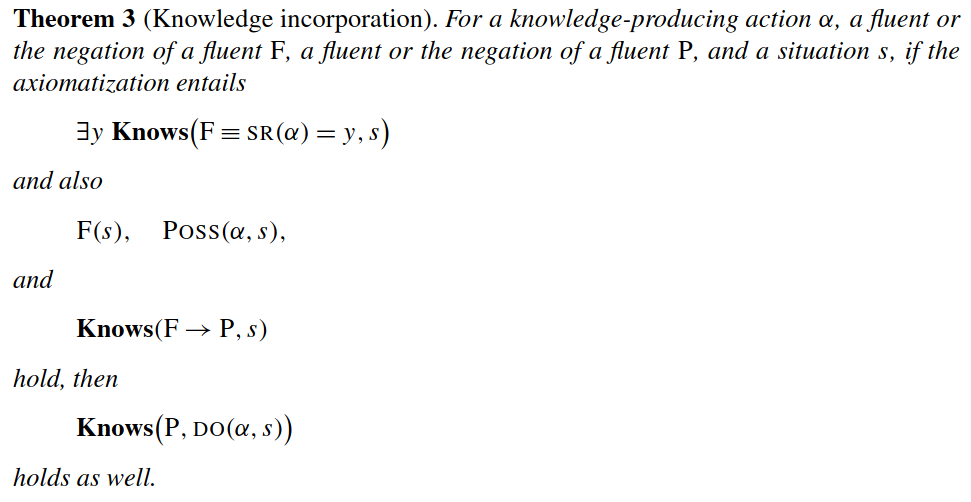
\includegraphics[width=0.7\textwidth]{assets/theorem3.png}
    \end{center}
\end{frame} 

\begin{frame}{Theorems}
    \begin{center}
        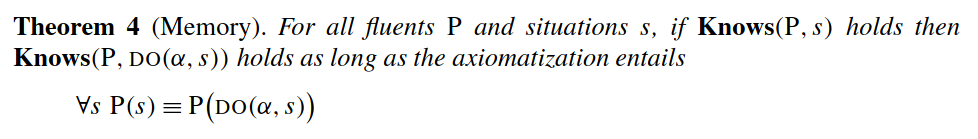
\includegraphics[width=0.7\textwidth]{assets/theorem4.png}
        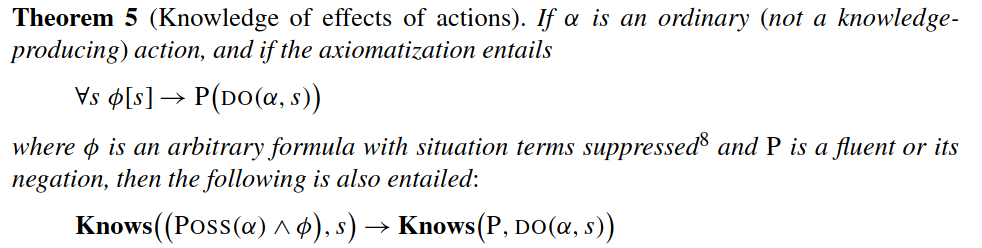
\includegraphics[width=0.7\textwidth]{assets/theorem5.png}
    \end{center}
\end{frame} 

\subsection{Regression}

\begin{frame}{Reasoning Tasks}
    \vspace*{-0.5cm}
    \begin{block}{Projection Task}
        Determing if a sentence G is true in the situation resulting
        from the execution of an action sequence is represented by the query:
            \[ \textit{F} \models \textit{G}(\text{DO}([\alpha_1, \ldots, \alpha_{n}], S_0)) \]
            %\[ \knows(\textfluent{P}, S1) \land \lnot \knows(\textfluent{Q}, S1) \]
    \end{block}
    \begin{block}{Legality Task}<2->
        The situation term
            \[ \text{DO}(\alpha_m, \text{DO}(\alpha_{m-1} \ldots \text{DO}(\alpha_1, S_0) \ldots)) \]
        is a legal situation iff 
            \[ [\alpha_1, \ldots, \alpha_{m}] \]
        is a legal action sequence        
    \end{block}    
\end{frame}

\begin{frame}{Regression}
 
    \begin{itemize}
    \item Reduce Reasoning about future situations to reasoning about the initial situation;
    \item Sound and Complete Reasoner.
    \end{itemize}

    \end{frame}

    \begin{frame}{Regression}

    Definition of Regressor Operator through:    

    \begin{itemize}
    \item Ordinary Actions
    \item Knowledge-Producing Actions
    %\item<1->
    \end{itemize}

\end{frame}       

\begin{frame}{Regression Theorem}
    \begin{theorem}
     For any ground situation term 
     \[ \textit{F} \models \textit{G}(s_{gr}) \quad iff \quad \textit{F} - \textit{F}_{\textit{SS}} \models \text{R}^*_{\theta}[\textit{G}(s_{gr})] \] 
    \end{theorem}
    \begin{proof}
     It suffices to show the preservation of logical equivalence
     \[ \textit{F} \ \models \textit{G}(s_{gr}) \ \equiv \ \text{R}^*_{\theta}[\textit{G}(s_{gr})] \]   
    \end{proof}        
\end{frame}     

\begin{frame}{Regression Theorem}
    \begin{theorem}[Regression-Ordinary Actions]
        \[ \text{R}^*_{\theta}[\knows(W, \text{DO}(a, s))] \equiv \]
            
        \[ \knows(\text{POSS}(a) \rightarrow \text{R}^*_{\theta}[W[\text{DO}(a, s')]], s) \]
        %  \textit{F} \models \Pi(\alpha_1)[s \rightarrow S_0] \land \Pi(\alpha_2)[s \rightarrow \text{DO}(\alpha_1, S_0)] \land \ldots \]
    \end{theorem}    
\end{frame}

\begin{frame}{Regression-Ordinary Actions}
    \begin{proof}  
       1. \ \knows(W, \text{DO}(a, s)) \\
       2. \ by the definition of \textbf{Knows}: \ \[ \forall s'' \  \text{K}(s'', \text{DO}(a, s)) \ \rightarrow \text{W}[s''] \] \\
    \end{proof} 
\end{frame} 

\begin{frame}{Regression-Ordinary Actions}
    \begin{proof}  
       3. \ by Successor State Axiom: \[ \text{K}(s'', \text{DO}(a, s)) \ \equiv \ \exists s'(\text{K}(s',s) \land \text{POSS}(a, s) \land s'' = \text{DO}(a, s'))\]
          \[ \forall s''(\exists s'(\text{K}(s',s) \land \text{POSS}(a, s') \land s'' = \text{DO}(a, s')) \rightarrow \text{W}[s''])  \]
       4. \ the axiomatization entails: \[ \forall s,s' \text{SR}(a, s) = \text{SR}(a, s') \] 
          \[ \forall s'(\text{K}(s',s) \land \text{POSS}(a, s') \rightarrow W[\text{DO}(a, s')]) \]
    \end{proof}
\end{frame}

\begin{frame}{Regression-Ordinary Actions}

    \begin{proof}  
       5. \ Inductive Hypothesis: \[ \forall s'(\text{K}(s',s) \land (\text{POSS}(a, s'))) \rightarrow \text{R}_{\theta}[W[\text{DO}(a, s')]] \] \\
          \ \[ \forall s'(\text{K}(s',s) \land (\text{POSS}(a, s'))) \rightarrow \text{R}_{\theta}[W[\text{DO}(a, s')]]^{-1} \] \\
       
       6. \ again by definition of \textbf{Knows}: \  \[ \knows(\text{POSS}(a) \rightarrow \text{R}_{\theta}[W[\text{DO}(a, s')]]^{-1}, s) \]
    \end{proof} 

\end{frame}


\begin{frame}{Regression Theorem}

\begin{theorem}[Regression- Knowledge Producing Actions]

    \[ \text{R}_{\theta}[\knows(W, \text{DO}(\text{SENSE}_i, s))] = \]
    \[ \exists y \ \text{SR}(\text{SENSE}_i, s) = y \ \land \]       
    \[ \knows((\text{POSS}(a) \land \text{SR}(\text{SENSE}_i) = y) \rightarrow \text{R}_{\theta}[W[\text{DO}(\text{SENSE}_i)]]^{-1}, s) \]
          %  \textit{F} \models \Pi(\alpha_1)[s \rightarrow S_0] \land \Pi(\alpha_2)[s \rightarrow \text{DO}(\alpha_1, S_0)] \land \ldots \]
          %\( \exists x \, P(x) \)
\end{theorem}      
\end{frame}

\begin{frame}{Regression- Knowledge Producing Actions}

    \begin{center}
        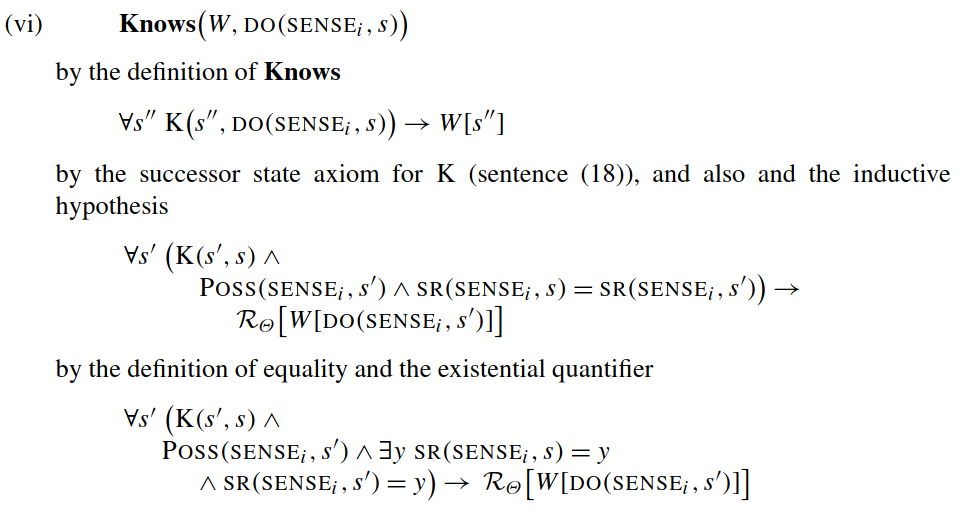
\includegraphics[width=0.7\textwidth]{assets/proof1.png}
    \end{center}

\end{frame}

\begin{frame}{Regression- Knowledge Producing Actions}

    \begin{center}
        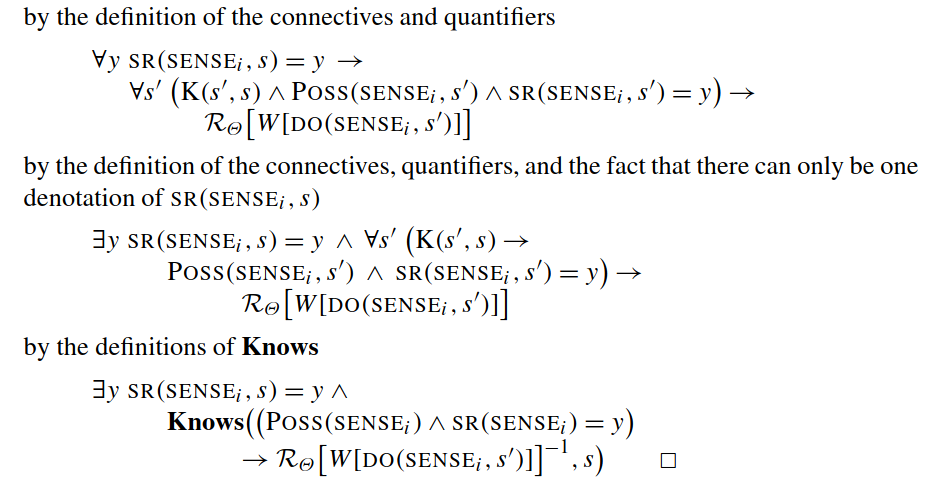
\includegraphics[width=0.7\textwidth]{assets/proof2.png}
    \end{center}

\end{frame}

\begin{frame}{Legality Testing}
    \vspace*{-0.5cm}
    \begin{block}{Method}
    \raggedright
    Given \textit{n} actions, the action precondition axioms are:
        \centering $ \forall x_n \text{ POSS}(A_n(x_n), s) \equiv \Pi A_n(x_n, s) $ \\ 
    \raggedright
    A sequence is a legal action sequence iff:     
        \[ \textit{F} \models \Pi(\alpha_1)[s \rightarrow S_0] \land \Pi(\alpha_2)[s \rightarrow \text{DO}(\alpha_1, S_0)] \land \ldots \]
        \[ \land \Pi(\alpha_m)[s \rightarrow \text{DO}([\alpha_1, \ldots, \alpha_{m-1}], S_0)] \]
    So iff, by Regression:
        \[ \textit{F} - \textit{F}_{\textit{SS}} \models \Pi(\alpha_1)[s \rightarrow S_0] \land \text{R}^*_{\theta}[\Pi(\alpha_2)[s \rightarrow \text{DO}(\alpha_1, S_0)]] \land \ldots \]
        \[ \land \text{R}^*_{\theta}[\Pi(\alpha_m)[s \rightarrow \text{DO}([\alpha_1, \ldots, \alpha_{m-1}], S_0)]] \]
    \end{block}
\end{frame}
